


\chapter{Duality}\label{chap:duality}

This section will now establish the connection that exists between multi-paths and multi-surfaces that will henceforth be referred to as ``duality".


\section{Point-volume duality}

To quantify a multi-point \(\rho\), at each position \(\mathbf{q}\) only one value \(\rho(\mathbf{q})\) is required. 

To quantify a multi-volume \(U\), at each position \(\mathbf{q}\) only one value \(U(\mathbf{q})\) is also required. 

The fact that multi-points and multi-volumes both only require 1 value suggests that points and volumes can be ``interchanged". When a multi-point and a multi-volume are interchangeable, they will be referred to as being ``dual" to each other.

\begin{tabular}{cc}
\parbox{0.5\textwidth}{
Given a point \(P\) with an {\bf infinitesimal} weight of \(w\), then the volume that is ``dual" to \(P\) is an infinitesimal volume \(\Omega\) that both contains \(P\) and has a volume of \(w\). 

Given an {\bf infinitesimal} volume \(\Omega\) with a volume of \(\Delta V\), then the point that is ``dual" to \(\Omega\) is a point \(P\) that is contained by \(\Omega\) and has a weight of \(\Delta V\).

Consider a multi-volume \(U\). Multi-volume \(U\) consists of a single volume with a weight of \(1\). The multi-point \(\rho\) that is ``dual" to \(\Omega\) is a uniform ``cloud" of points each with an infinitesimal weight. The average total weight per unit volume is \(1\). In the image on the right, a large volume is shattered into infinitesimal volumes, each shard of which is dual to point with a weight equal to the volume of said shard. 
} & \parbox{0.5\textwidth}{
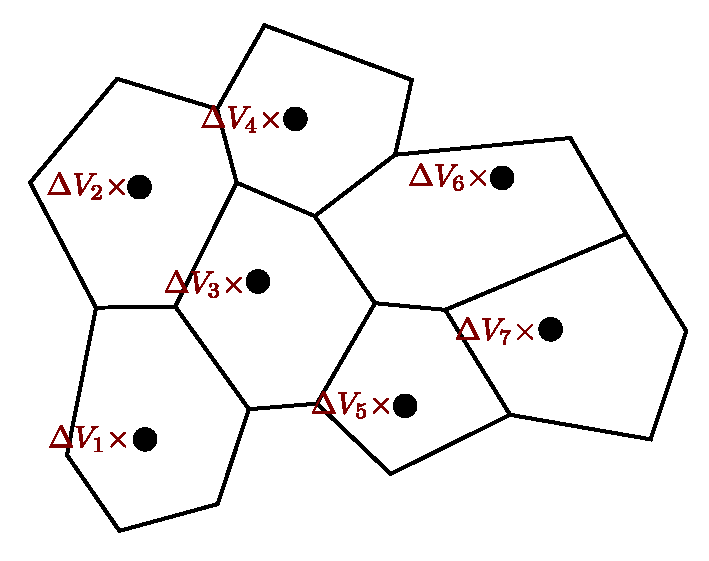
\includegraphics[width = 0.5\textwidth]{Duality/point_volume_duality}
}
\end{tabular}

While there is no unique way of exactly placing the dual points or sketching the dual volumes, once ``smoothing" has been applied none of this matters.

Given a multi-volume \(U\), the multi-point \(\rho\) that is ``dual" to \(U\) will be denoted via the notation:
\[\rho = \iota(U)\]
or conversely, 
\[U = \iota^{-1}(\rho)\]

The following is important to note:
\begin{itemize}
\item The dual of the union is the union of the duals:
\[\iota(U_1 + U_2) = \iota(U_1) + \iota(U_2)
\quad\quad\text{and}\quad\quad
\iota^{-1}(\rho_1 + \rho_2) = \iota^{-1}(\rho_1) + \iota^{-1}(\rho_2)\]
If \(c\) is an arbitrary real valued coefficient, then:
\[\iota(c \cdot U) = c \cdot \iota(U)
\quad\quad\text{and}\quad\quad
\iota^{-1}(c \cdot \rho) = c \cdot \iota^{-1}(\rho)\]
\end{itemize}




\section{Path-surface duality}

To quantify a multi-path \(\mathbf{J}\), at each position \(\mathbf{q}\) three values \(\begin{bmatrix} J_1(\mathbf{q}) \\ J_2(\mathbf{q}) \\ J_3(\mathbf{q}) \end{bmatrix}\) are required. 

To quantify a multi-surface \(\mathbf{F}\), at each position \(\mathbf{q}\) three values \(\begin{bmatrix} F_1(\mathbf{q}) \\ F_2(\mathbf{q}) \\ F_3(\mathbf{q}) \end{bmatrix}\) are also required. 

The fact that multi-paths and multi-surface both require 3 values suggests that paths and surfaces can be ``interchanged". When a multi-path and multi-surface are interchangeable, they will be referred to as being ``dual" to each other.

Given an infinitesimal segment of path \(C\) with an infinitesimal weight, the surface \(\sigma\) that is ``dual" to \(C\) is: 
\begin{itemize}
\item Infinitesimal in both size and weight.
\item Perpendicular to \(C\). 
\item The direction of \(C\) passes through \(\sigma\) in the preferred direction. This gives the intersections of dual paths and surfaces positive weight. 
\end{itemize}

To visualize a smoothed multi-path and its smoothed dual surface, sheath the infinitesimal path fibers in a cylinder. The path fibers are parallel to the sides of the cylinder, and are perpendicular to the end caps. The dual surfaces are perpendicular to the sides of the cylinder and are parallel to the end caps. The total path weight passing through the cylinder is proportional to the cross-sectional area of the cylinder, while the total surface weight slicing through the cylinder is proportional to its length.

In the image below, the leftmost cylinders contain a path with a total weight of \(w_{\parallel}\), and a surface with a total weight of \(w_{\perp}\). These paths and surfaces are dual to each other. In the top row of images, when the cylinder decreases in length, the contained surface weight decreases proportionally, while the contained path weight remains constant. In the bottom row of images, when the cylinder decreases in cross-sectional area, the contained path weight decreases proportionally, while the contained surface weight remains constant. 

\begin{center}
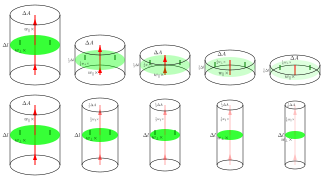
\includegraphics[width = 0.9\textwidth]{Duality/path_surface_duality_2}
\end{center}

To determine the multi-path \(\mathbf{J}\) that is dual to a multi-surface \(\mathbf{F}\), break the multi-surface \(\mathbf{F}\) into infinitesimal sections with equal weight and area, replace each section of surface with its dual path, and lastly stitch the path segments together leaving as little endpoints as possible. While there is no unique way of performing this process, once ``smoothing" has been applied none of this matters.  

\begin{center}
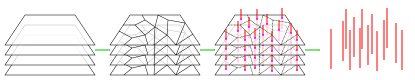
\includegraphics[width = 0.9\textwidth]{Duality/path_surface_duality_3}
\end{center}

Given a multi-surface \(\mathbf{F}\), the multi-path \(\mathbf{J}\) that is ``dual" to \(\mathbf{F}\) will be denoted via the notation:
\[\mathbf{J} = \epsilon(\mathbf{F})\]
or conversely, 
\[\mathbf{F} = \epsilon^{-1}(\mathbf{J})\]

The following is important to note:
\begin{itemize}
\item The dual of the union is the union of the duals:
\[\epsilon(\mathbf{F}_1 + \mathbf{F}_2) = \epsilon(\mathbf{F}_1) + \epsilon(\mathbf{F}_2)
\quad\quad\text{and}\quad\quad
\epsilon^{-1}(\mathbf{J}_1 + \mathbf{J}_2) = \epsilon^{-1}(\mathbf{J}_1) + \epsilon^{-1}(\mathbf{J}_2)\]
If \(c\) is an arbitrary real valued coefficient, then:
\[\epsilon(c \cdot \mathbf{F}) = c \cdot \epsilon(\mathbf{F})
\quad\quad\text{and}\quad\quad
\epsilon^{-1}(c \cdot \mathbf{J}) = c \cdot \epsilon^{-1}(\mathbf{J})\]
\end{itemize}



\section{Duality and intersections}

\begin{thm}
Given multi-point \(\rho\) and multi-volume \(V\), 

\[\iota^{-1}(\rho \cdot V) = \iota^{-1}(\rho) \cdot V\]

Given multi-point \(\mathbf{J}\) and multi-volume \(V\), 

\[\epsilon^{-1}(\mathbf{J} \cdot V) = \epsilon^{-1}(\mathbf{J}) \cdot V\]

Given multi-surface \(\mathbf{F}\) and multi-volume \(V\), 

\[\epsilon(\mathbf{F} \cdot V) = \epsilon(\mathbf{F}) \cdot V\]

Given multi-volume \(U\) and multi-volume \(V\), 

\[\iota(U \cdot V) = \iota(U) \cdot V\]
\end{thm}


\begin{tabular}{cc}
\parbox{0.5\textwidth}{
\begin{thm}\label{thm:point-volume_intersection_duality}
Given multi-volumes \(U\) and \(V\), 
\[\iota(U) \cdot V = U \cdot \iota(V)\]
\end{thm}
\textbf{Proof:}

Let \(u\) and \(v\) be infinitesimally small single volumes with weights of \(1\), and whose volumes are equivalent. There are two scenarios. In the first scenario, \(\iota(u)\) and \(\iota(v)\) are at different positions. In the second scenario, \(\iota(u) = \iota(v)\). These scenarios are depicted on the right.

\begin{itemize}
\item In case 1, \(\iota(u) \cdot v = 0\) and \(u \cdot \iota(v) = 0\) so \(\iota(u) \cdot v = u \cdot \iota(v)\). 
\item In case 2, \(\iota(u) = \iota(v)\) implies \(u = v\). Therefore \(\iota(u) \cdot v = u \cdot \iota(v)\).  
\end{itemize}
} & \parbox{0.5\textwidth}{
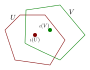
\includegraphics[width = 0.5\textwidth]{Duality/point_volume_duality_intersection}
}
\end{tabular}

For infinitesimal single volumes \(u\) and \(v\) with equal volumes and weights of \(1\), \(\iota(u) \cdot v = u \cdot \iota(v)\). Generalizing to non-infinitesimal scales, let \(U\) and \(V\) denote non-infinitesimal volumes comprised of infinitesimal volumes:
\[U = u_1 + u_2 + ... + u_{\infty}\] 
\[V = v_1 + v_2 + ... + v_{\infty}\]
Next:
\begin{align*}
\iota(U) \cdot V
= & \iota(u_1 + u_2 + ... + u_{\infty}) \cdot (v_1 + v_2 + ... + v_{\infty}) \\
= & (\iota(u_1) + \iota(u_2) + ... + \iota(u_{\infty})) \cdot (v_1 + v_2 + ... + v_{\infty}) \\  
= & \quad \iota(u_1) \cdot v_1 + \iota(u_1) \cdot v_2 + ... + \iota(u_1) \cdot v_\infty \\  
& + \iota(u_2) \cdot v_1 + \iota(u_2) \cdot v_2 + ... + \iota(u_2) \cdot v_\infty \\  
& ... \\
& + \iota(u_\infty) \cdot v_1 + \iota(u_\infty) \cdot v_2 + ... + \iota(u_\infty) \cdot v_\infty   
\end{align*}
\begin{align*}
= & \quad u_1 \cdot \iota(v_1) + u_1 \cdot \iota(v_2) + ... + u_1 \cdot \iota(v_\infty) \\ 
& + u_2 \cdot \iota(v_1) + u_2 \cdot \iota(v_2) + ... + u_2 \cdot \iota(v_\infty) \\ 
& ... \\ 
& + u_\infty \cdot \iota(v_1) + u_\infty \cdot \iota(v_2) + ... + u_\infty \cdot \iota(v_\infty) \\ 
= & (u_1 + u_2 + ... + u_\infty) \cdot (\iota(v_1) + \iota(v_2) + ... + \iota(v_\infty)) \\ 
= & (u_1 + u_2 + ... + u_\infty) \cdot \iota(v_1 + v_2 + ... + v_\infty) \\ 
= & U \cdot \iota(V)
\end{align*}
Therefore:
\[\iota(U) \cdot V = U \cdot \iota(V)\]
\(\Box\)



\begin{tabular}{cc}
\parbox{0.5\textwidth}{
\begin{thm}\label{thm:path-surface_intersection_duality}
Given multi-surfaces \(\mathbf{F}\) and \(\mathbf{G}\), 
\[\epsilon(\mathbf{F}) \bullet \mathbf{G} = \mathbf{F} \bullet \epsilon(\mathbf{G})\]
\end{thm}
\textbf{Proof:}

Let \(\mathbf{f}\) and \(\mathbf{g}\) be infinitesimally small surfaces with weights of \(w_{\perp}\). Let the dual paths \(\epsilon(\mathbf{f})\) and \(\epsilon(\mathbf{g})\) have weights of \(w_{\parallel}\). There are two scenarios. In the first scenario, \(\mathbf{f}\) and \(\mathbf{g}\) are at different positions. In the second scenario, \(\mathbf{f}\) and \(\mathbf{g}\) are at the same position. These scenarios are depicted on the right.

\begin{itemize}
\item In case 1, \(\epsilon(\mathbf{f}) \bullet \mathbf{g} = 0\) and \(\mathbf{f} \cdot \epsilon(\mathbf{g}) = 0\) so \(\epsilon(\mathbf{f}) \bullet \mathbf{g} = \mathbf{f} \cdot \epsilon(\mathbf{g})\). 
\item In case 2, the intersection point \(\epsilon(\mathbf{f}) \bullet \mathbf{g}\) has a weight of \(w_{\parallel} w_{\perp}\). The intersection point \(\mathbf{f} \bullet \epsilon(\mathbf{g})\) also has a weight of \(w_{\parallel} w_{\perp}\), and has the same position. Therefore \(\epsilon(\mathbf{f}) \bullet \mathbf{g} = \mathbf{f} \bullet \epsilon(\mathbf{g})\).  
\end{itemize}
} & \parbox{0.5\textwidth}{
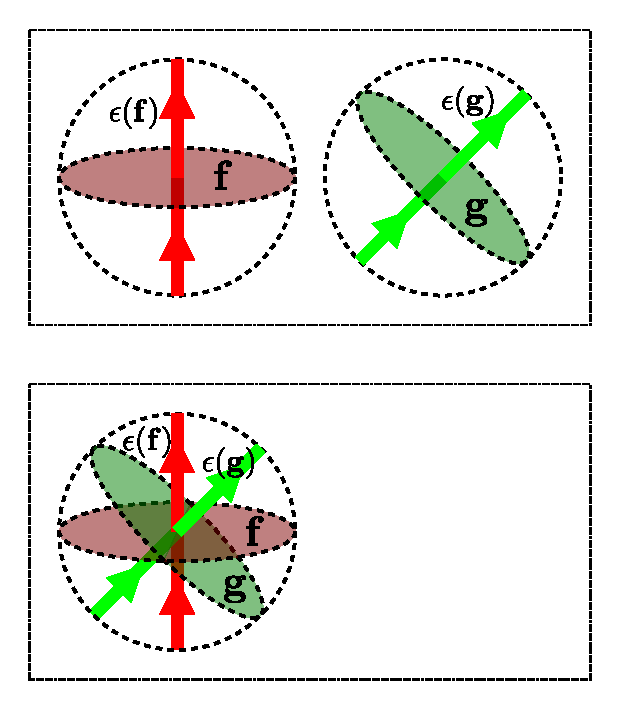
\includegraphics[width = 0.5\textwidth]{Duality/path_surface_duality_intersection}
}
\end{tabular}

For infinitesimal surfaces \(\mathbf{f}\) and \(\mathbf{g}\) with equal weights, \(\epsilon(\mathbf{f}) \bullet \mathbf{g} = \mathbf{f} \bullet \epsilon(\mathbf{g})\). Generalizing to non-infinitesimal scales, let \(\mathbf{F}\) and \(\mathbf{G}\) denote non-infinitesimal volumes comprised of infinitesimal volumes:
\[\mathbf{F} = \mathbf{f}_1 + \mathbf{f}_2 + ... + \mathbf{f}_{\infty}\] 
\[\mathbf{G} = \mathbf{g}_1 + \mathbf{g}_2 + ... + \mathbf{g}_{\infty}\]
Next:
\begin{align*}
\epsilon(\mathbf{F}) \bullet \mathbf{G} 
= & \epsilon(\mathbf{f}_1 + \mathbf{f}_2 + ... + \mathbf{f}_{\infty}) \bullet (\mathbf{g}_1 + \mathbf{g}_2 + ... + \mathbf{g}_{\infty}) \\
= & (\epsilon(\mathbf{f}_1) + \epsilon(\mathbf{f}_2) + ... + \epsilon(\mathbf{f}_{\infty})) \bullet (\mathbf{g}_1 + \mathbf{g}_2 + ... + \mathbf{g}_{\infty}) \\  
= & \quad \epsilon(\mathbf{f}_1) \bullet \mathbf{g}_1 + \epsilon(\mathbf{f}_1) \bullet \mathbf{g}_2 + ... + \epsilon(\mathbf{f}_1) \bullet \mathbf{g}_\infty \\  
& + \epsilon(\mathbf{f}_2) \bullet \mathbf{g}_1 + \epsilon(\mathbf{f}_2) \bullet \mathbf{g}_2 + ... + \epsilon(\mathbf{f}_2) \bullet \mathbf{g}_\infty \\  
& ... \\
& + \epsilon(\mathbf{f}_\infty) \bullet \mathbf{g}_1 + \epsilon(\mathbf{f}_\infty) \bullet \mathbf{g}_2 + ... + \epsilon(\mathbf{f}_\infty) \bullet \mathbf{g}_\infty   
\end{align*}
\begin{align*}
= & \quad \mathbf{f}_1 \bullet \epsilon(\mathbf{g}_1) + \mathbf{f}_1 \bullet \epsilon(\mathbf{g}_2) + ... + \mathbf{f}_1 \bullet \epsilon(\mathbf{g}_\infty) \\  
& + \mathbf{f}_2 \bullet \epsilon(\mathbf{g}_1) + \mathbf{f}_2 \bullet \epsilon(\mathbf{g}_2) + ... + \mathbf{f}_2 \bullet \epsilon(\mathbf{g}_\infty) \\  
& ... \\
& + \mathbf{f}_\infty \bullet \epsilon(\mathbf{g}_1) + \mathbf{f}_\infty \bullet \epsilon(\mathbf{g}_2) + ... + \mathbf{f}_\infty \bullet \epsilon(\mathbf{g}_\infty) \\  
= & (\mathbf{f}_1 + \mathbf{f}_2 + ... + \mathbf{f}_\infty) \bullet (\epsilon(\mathbf{g}_1) + \epsilon(\mathbf{g}_2) + ... + \epsilon(\mathbf{g}_\infty)) \\ 
= & (\mathbf{f}_1 + \mathbf{f}_2 + ... + \mathbf{f}_\infty) \bullet \epsilon(\mathbf{g}_1 + \mathbf{g}_2 + ... + \mathbf{g}_\infty) \\ 
= & \mathbf{F} \bullet \epsilon(\mathbf{G})
\end{align*}
Therefore:
\[\epsilon(\mathbf{F}) \bullet \mathbf{G} = \mathbf{F} \bullet \epsilon(\mathbf{G})\]
\(\Box\)



%Given multi-paths \(\mathbf{J}\) and \(\mathbf{K}\), and multi-surface \(\mathbf{F}\), then:
%
%\[\mathbf{F} \times \epsilon^{-1}(\epsilon^{-1}(\mathbf{J}) \times \epsilon^{-1}(\mathbf{K})) = \iota^{-1}(\mathbf{F} \bullet \mathbf{K})\mathbf{J} - \iota^{-1}(\mathbf{F} \bullet \mathbf{J})\mathbf{K}\]
%
%\begin{tabular}{cc}
%\parbox{0.5\textwidth}{
%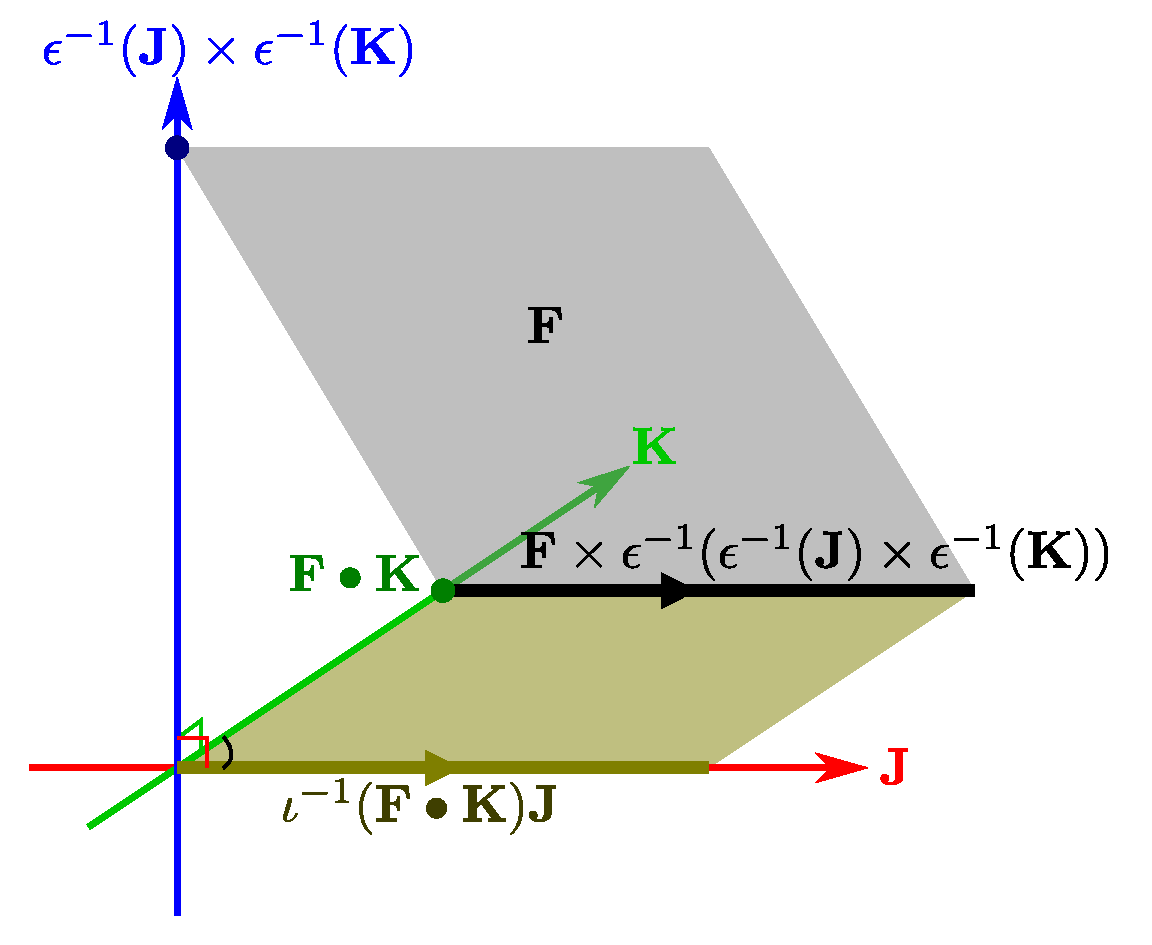
\includegraphics[width = 0.5\textwidth]{Duality/triple_vector_product_tetrahedron_F_dot_J=0}
%} & \parbox{0.5\textwidth}{
%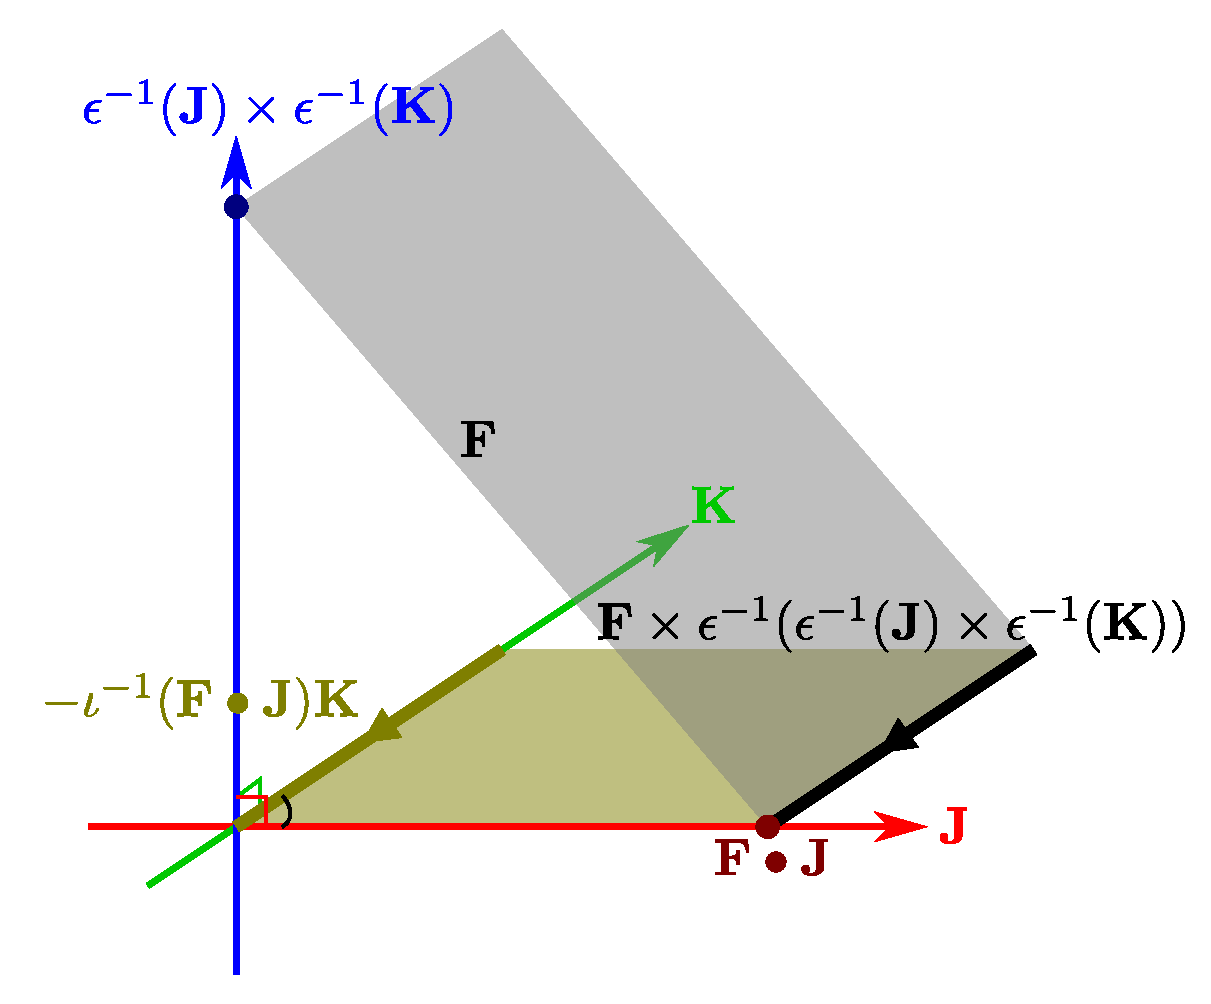
\includegraphics[width = 0.5\textwidth]{Duality/triple_vector_product_tetrahedron_F_dot_K=0}
%} 
%\end{tabular}
%
%\begin{center}
%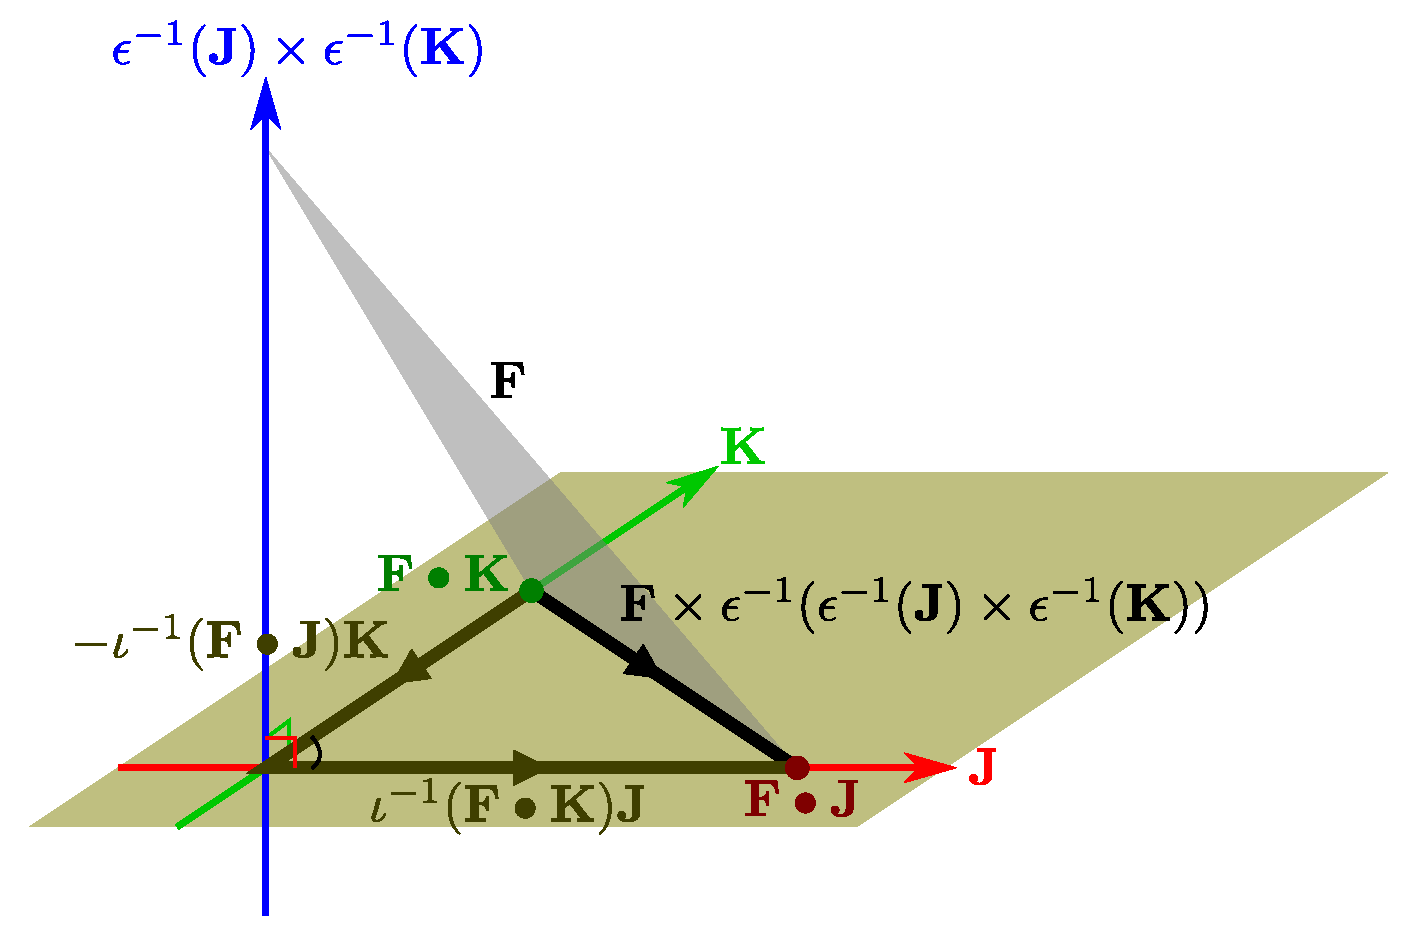
\includegraphics[width = 0.75\textwidth]{Duality/triple_vector_product_tetrahedron}
%\end{center}



\section{Simplifying notation}

In the discussions that will follow, duality conversions will begin to happen rapidly, and to avoid notational clutter, the following abbreviations will be made:

\begin{itemize}
%%%%%
\item Given multi-points \(\rho_1\) and \(\rho_2\), the expression \(\rho_1 \cdot \rho_2\) will be defined by  
\[\rho_1 \cdot \rho_2 = \iota^{-1}(\rho_1) \cdot \rho_2 = \rho_1 \cdot \iota^{-1}(\rho_2)\]
Thanks to theorem \ref{thm:point-volume_intersection_duality}, \(\iota^{-1}(\rho_1) \cdot \rho_2 = \rho_1 \cdot \iota^{-1}(\rho_2)\)
%%%%%
\item Given multi-point \(\rho\) and multi-path \(\mathbf{J}\), the expression \(\rho \cdot \mathbf{J}\) will be defined by
\[\rho \cdot \mathbf{J} = \iota^{-1}(\rho) \cdot \mathbf{J}\]
%%%%%
\item Given multi-point \(\rho\) and multi-surface \(\mathbf{F}\), the expression \(\rho \cdot \mathbf{F}\) will be defined by
\[\rho \cdot \mathbf{F} = \iota^{-1}(\rho) \cdot \mathbf{F}\]
%%%%%
\item Given multi-paths \(\mathbf{J}_1\) and \(\mathbf{J}_2\), the expression \(\mathbf{J}_1 \bullet \mathbf{J}_2\) will be defined by 
\[\mathbf{J}_1 \bullet \mathbf{J}_2 = \epsilon^{-1}(\mathbf{J}_1) \bullet \mathbf{J}_2 = \mathbf{J}_1 \bullet \epsilon^{-1}(\mathbf{J}_2)\]
Thanks to theorem \ref{thm:path-surface_intersection_duality}, \(\epsilon^{-1}(\mathbf{J}_1) \bullet \mathbf{J}_2 = \mathbf{J}_1 \bullet \epsilon^{-1}(\mathbf{J}_2)\)
%%%%%
\item Given multi-surfaces \(\mathbf{F}_1\) and \(\mathbf{F}_2\), the expression \(\mathbf{F}_1 \bullet \mathbf{F}_2\) will be defined by 
\[\mathbf{F}_1 \bullet \mathbf{F}_2 = \epsilon(\mathbf{F}_1) \bullet \mathbf{F}_2 = \mathbf{F}_1 \bullet \epsilon(\mathbf{F}_2)\]
Thanks to theorem \ref{thm:path-surface_intersection_duality}, \(\epsilon(\mathbf{F}_1) \bullet \mathbf{F}_2 = \mathbf{F}_1 \bullet \epsilon(\mathbf{F}_2)\)
%%%%%
\item Given multi-paths \(\mathbf{J}_1\) and \(\mathbf{J}_2\), the expression \(\mathbf{J}_1 \times \mathbf{J}_2\) will be defined by 
\[\mathbf{J}_1 \times \mathbf{J}_2 = \epsilon^{-1}(\mathbf{J}_1) \times \epsilon^{-1}(\mathbf{J}_2)\]
%%%%%
\item Given multi-path \(\mathbf{J}\) and multi-surface \(\mathbf{F}\), the expression \(\mathbf{J} \times \mathbf{F}\) will be defined by 
\[\mathbf{J} \times \mathbf{F} = \epsilon^{-1}(\mathbf{J}) \times \mathbf{F}\]
%%%%%
\item Given multi-surface \(\mathbf{F}\) and multi-path \(\mathbf{J}\), the expression \(\mathbf{F} \times \mathbf{J}\) will be defined by 
\[\mathbf{F} \times \mathbf{J} = \mathbf{F} \times \epsilon^{-1}(\mathbf{J})\]
%%%%%
\item Given multi-point \(\rho\), the expression \(\nabla \rho\) will be defined by 
\[\nabla \rho = \nabla \iota^{-1}(\rho)\]
%%%%%
\item Given multi-path \(\mathbf{J}\), the expression \(\nabla \times \mathbf{J}\) will be defined by 
\[\nabla \times \mathbf{J} = \nabla \times \epsilon^{-1}(\mathbf{J})\]
%%%%%
\item Given multi-surface \(\mathbf{F}\), the expression \(\nabla \bullet \mathbf{F}\) will be defined by 
\[\nabla \bullet \mathbf{F} = \nabla \bullet \epsilon(\mathbf{F})\]
\item Given multi-volume \(U\), the expression \(\int U\) will be defined by
\[\int U = \int \iota(U)\]
This expression computes the total volume of \(U\).
\end{itemize}

{\bf In summary, if an operation cannot be performed, compute the dual of one (or both) of the operands until the operation is possible.}


\section{Energy}

\subsection{Path energy}

Given a multi-path \(\mathbf{D}\), the ``energy" of \(\mathbf{D}\) is \(1/2\) the total number of intersections that the path has with its own dual:

\[E = \frac{1}{2}\int (\mathbf{D} \bullet \mathbf{D}) = \frac{1}{2}\int (\mathbf{D} \bullet \epsilon^{-1}(\mathbf{D}))\]

The multiplier of \(\frac{1}{2}\) exists to remain consistent with physics.

The energy is always strictly positive except for the \(0\) multi-path where the energy is \(0\).


\subsection{Surface energy}

Given a multi-surface \(\mathbf{E}\), the ``energy" of \(\mathbf{E}\) is \(1/2\) the total number of intersections that the surface has with its own dual:

\[E = \frac{1}{2}\int (\mathbf{E} \bullet \mathbf{E}) = \frac{1}{2}\int (\epsilon(\mathbf{E}) \bullet \mathbf{E})\]

Again, the multiplier of \(\frac{1}{2}\) exists to remain consistent with physics.

The energy is always strictly positive except for the \(0\) multi-surface where the energy is \(0\).


\subsection{Loop-bubble duality}


If a multi-bubble is dual to a multi-loop, then both are \(0\). This can be proven from  the fact that the energy of a nonzero path or surface is always positive. 

\begin{thm}\label{thm:loop_bubble_duality}
Assume that \(\mathbf{E}\) is a multi-bubble: \(\nabla \times \mathbf{E} = 0\). Also assume that the dual multi-path \(\mathbf{D} = \epsilon(\mathbf{E})\) is also a multi-loop: \(\nabla \bullet \mathbf{D} = 0\). It must then be the case that \(\mathbf{E} = 0\) and \(\mathbf{D} = 0\).
\end{thm}
\textbf{Proof:}

Since \(\mathbf{E}\) is a multi-bubble, there must exist some multi-volume \(U\) whose inwards oriented surface is \(\mathbf{E}\). 

The energy of both \(\mathbf{D}\) and \(\mathbf{E}\) is:

\begin{align*}
E = & \frac{1}{2}\int (\mathbf{D} \bullet \mathbf{E}) 
= \frac{1}{2} \int (\mathbf{D} \bullet (\nabla U)) 
\end{align*} 

As established by theorem \ref{thm:gradient_theorem}, the number of times \(\mathbf{D}\) enters \(U\) is the total number of finishing points \(\mathbf{D}\) leaves in \(U\) so: 
\[\int (\mathbf{D} \bullet (\nabla U)) = -\int ((\nabla \bullet \mathbf{D}) U)\] 
therefore continuing the derivation yields:

\begin{align*}
E = & \frac{1}{2} \int (\mathbf{D} \bullet (\nabla U)) 
= -\frac{1}{2} \int ((\nabla \bullet \mathbf{D}) U) 
= -\frac{1}{2} \int (0 \cdot U) 
= 0
\end{align*}

The energy is \(0\), and this only occurs if \(\mathbf{D} = 0\) and \(\mathbf{E} = 0\). {\bf Non-zero multi-bubbles can never be dual to a multi-loop and vice versa. \(\Box\)}


A consequence of this fact is that if two path-surface pairs have the same end-points and counterclockwise boundaries, then they are equivalent: 

\begin{cor}\label{cor:loop_bubble_duality}
Let \(\mathbf{D}_1\) and \(\mathbf{E}_1\) be a multi-path and a multi-surface pair that are dual to each other: \(\mathbf{D}_1 = \epsilon(\mathbf{E}_1)\)

Let \(\mathbf{D}_2\) and \(\mathbf{E}_2\) also be a multi-path and a multi-surface pair that are dual to each other: \(\mathbf{D}_2 = \epsilon(\mathbf{E}_2)\)

If \(\nabla \bullet \mathbf{D}_1 = \nabla \bullet \mathbf{D}_2\) and \(\nabla \times \mathbf{E}_1 = \nabla \times \mathbf{E}_2\), then \(\mathbf{D}_1 = \mathbf{D}_2\) and \(\mathbf{E}_1 = \mathbf{E}_2\).   
\end{cor}
\textbf{Proof:}

Let \(\mathbf{D}_{\text{loop}} = \mathbf{D}_1 - \mathbf{D}_2\). \(\mathbf{D}_{\text{loop}}\) is a multi-loop:
\[\nabla \bullet \mathbf{D}_{\text{loop}} = \nabla \bullet (\mathbf{D}_1 - \mathbf{D}_2) = \nabla \bullet \mathbf{D}_1 - \nabla \bullet \mathbf{D}_2 = 0\]

Let \(\mathbf{E}_{\text{bubble}} = \mathbf{E}_1 - \mathbf{E}_2\). \(\mathbf{E}_{\text{bubble}}\) is a multi-bubble: 
\[\nabla \times \mathbf{E}_{\text{bubble}} = \nabla \times (\mathbf{E}_1 - \mathbf{E}_2) = \nabla \times \mathbf{E}_1 - \nabla \times \mathbf{E}_2 = 0\]

\(\mathbf{D}_{\text{loop}}\) and \(\mathbf{E}_{\text{bubble}}\) are a dual pair:
\[\epsilon(\mathbf{E}_{\text{bubble}}) = \epsilon(\mathbf{E}_1 - \mathbf{E}_2) = \epsilon(\mathbf{E}_1) - \epsilon(\mathbf{E}_2) = \mathbf{D}_1 - \mathbf{D}_2 = \mathbf{D}_{\text{loop}}\]

From theorem \ref{thm:loop_bubble_duality}, \(\mathbf{D}_{\text{loop}} = 0\) and \(\mathbf{E}_{\text{bubble}} = 0\). Therefore \(\mathbf{D}_1 = \mathbf{D}_2\) and \(\mathbf{E}_1 = \mathbf{E}_2\). \(\Box\)



\subsection{Low energy multi-path}

Given a balanced multi-point \(\rho\), it is known via theorem \ref{thm:dot-to-dot} from section \ref{sec:balanced_multi-points} that there must exist a multi-path \(\mathbf{D}\) such that \(\nabla \bullet \mathbf{D} = \rho\). However, the choice of \(\mathbf{D}\) is {\bf not unique}. A unique choice of multi-path \(\mathbf{D}\) is the choice that minimizes the energy \(\frac{1}{2}\int (\mathbf{D} \bullet \mathbf{D})\). It will now be demonstrated that the energy minimizing choice is both unique and is dual to a multi-bubble:

\begin{thm}
Given a balanced multi-point \(\rho\), the multi-path \(\mathbf{D}\) that satisfies \(\nabla \bullet \mathbf{D} = \rho\) and minimizes the energy \(\frac{1}{2}\int (\mathbf{D} \bullet \mathbf{D})\) is both {\bf unique} and is dual to a multi-bubble: i.e. \(\nabla \times \mathbf{D} = 0\). 
\end{thm}
\textbf{Proof:}

Let \(\mathbf{D}\) denote any multi-path whose endpoints are \(\rho\): \(\nabla \bullet \mathbf{D} = \rho\). It will be demonstrated that unless \(\nabla \times \mathbf{D} = 0\), that there will exist another multi-path \(\mathbf{D}_{\text{next}}\) whose endpoints are also \(\rho\): \(\nabla \bullet \mathbf{D}_{\text{next}} = \rho\), and has a lower energy than \(\mathbf{D}\). 

The approach that will be used here is referred to as the {\bf method of variations}. The method of variations involves proposing a change to \(\mathbf{D}\), and then determining conditions such that no changes result in lower energy. Choose any multi-surface \(\mathbf{F}\), referred to as a ``test surface". The boundary \(\nabla \times \mathbf{F}\) is a closed loop, and adding any multiple of \(\nabla \times \mathbf{F}\) to \(\mathbf{D}\) does not change the endpoints.

Let \(t\) be a small number (that is close to 0), and then propose the change:
\[\mathbf{D}_{\text{new}} = \mathbf{D} + t(\nabla \times \mathbf{F})\]
The endpoints are unchanged:
\begin{align*}
\nabla \bullet \mathbf{D}_{\text{new}} = & \nabla \bullet \mathbf{D} + t(\nabla \bullet (\nabla \times \mathbf{F})) \\ 
= & \nabla \bullet \mathbf{D} - t(0) 
= \rho
\end{align*}

The current energy is \(E_{\text{old}} = \frac{1}{2}\int (\mathbf{D} \bullet \mathbf{D})\)

The new energy is: 

\begin{align*}
E_{\text{new}} = & \frac{1}{2}\int (\mathbf{D}_{\text{new}} \bullet \mathbf{D}_{\text{new}}) \\ 
= & \frac{1}{2}\int (\mathbf{D} + t (\nabla \times \mathbf{F})) \bullet (\mathbf{D} + t (\nabla \times \mathbf{F})) \\ 
= & \frac{1}{2}\int (\mathbf{D} \bullet \mathbf{D} + t(\mathbf{D} \bullet (\nabla \times \mathbf{F}) + (\nabla \times \mathbf{F}) \bullet \mathbf{D}) + t^2((\nabla \times \mathbf{F}) \bullet (\nabla \times \mathbf{F}))) \\
= & \frac{1}{2}\int (\mathbf{D} \bullet \mathbf{D}) + t\int (\mathbf{D} \bullet (\nabla \times \mathbf{F})) + \frac{t^2}{2}\int ((\nabla \times \mathbf{F}) \bullet (\nabla \times \mathbf{F})) \\ 
= & E_{\text{old}} + t\int (\mathbf{D} \bullet (\nabla \times \mathbf{F})) + \frac{t^2}{2}\int ((\nabla \times \mathbf{F}) \bullet (\nabla \times \mathbf{F}))
\end{align*}

Of interest is the term \(\int (\mathbf{D} \bullet (\nabla \times \mathbf{F}))\). If this term is \(0\), then no choice of \(t\) results in lower energy. Contrariwise, if this term is non-zero, then \(t\) can be chosen to decrease the energy further. 

\(\int (\mathbf{D} \bullet (\nabla \times \mathbf{F}))\) is the total point weight of the intersection of the surface \(\epsilon^{-1}(\mathbf{D})\) with the counterclockwise boundary of \(\mathbf{F}\). Using Stokes' theorem (theorem \ref{thm:stokes_theorem}), 
\begin{align*}
& \int (\mathbf{D} \bullet (\nabla \times \mathbf{F})) = 0
\iff \int ((\nabla \times \mathbf{D}) \bullet \mathbf{F}) = 0 
\iff \int ((\nabla \times \mathbf{D}) \bullet \mathbf{F}) = \int (0 \bullet \mathbf{F}) 
\end{align*}

The energy cannot be reduced further if and only if \(\int (\mathbf{D} \bullet (\nabla \times \mathbf{F})) = 0\) for every choice of test surface \(\mathbf{F}\). Equivalently, the energy cannot be reduced further if and only if \(\int ((\nabla \times \mathbf{D}) \bullet \mathbf{F}) = \int (0 \bullet \mathbf{F})\) for every choice of test surface \(\mathbf{F}\).

Treat \(\mathbf{F}\) as a ``scanning window" from theorem \ref{thm:scanning_paths}. From this theorem, \(\int ((\nabla \times \mathbf{D}) \bullet \mathbf{F}) = \int (0 \bullet \mathbf{F})\) for every choice of scanning window \(\mathbf{F}\) if and only if \(\nabla \times \mathbf{D} = 0\). The energy cannot be reduced further if and only if \(\mathbf{D}\) is dual to a multi-bubble: i.e. \(\nabla \times \mathbf{D} = 0\).

It lastly needs to be demonstrated that the optimal choice of \(\mathbf{D}\) is unique. Let \(\mathbf{D}_1\) and \(\mathbf{D}_2\) denote two optimal choices of \(\mathbf{D}\). This means that \(\nabla \bullet \mathbf{D}_1 = \nabla \bullet \mathbf{D}_2 = \rho\) and \(\nabla \times \epsilon^{-1}(\mathbf{D}_1) = \nabla \times \epsilon^{-1}(\mathbf{D}_2) = 0\). From the corollary of theorem \ref{thm:loop_bubble_duality}, \(\mathbf{D}_1 = \mathbf{D}_2\). \(\Box\) 



\subsection{Low energy multi-surface}

Given a multi-loop \(\mathbf{J}\), it is known via theorem \ref{thm:filling_closed_loops} from section \ref{sec:closed_loops} that there must exist a multi-surface \(\mathbf{E}\) such that \(\nabla \times \mathbf{E} = \mathbf{J}\). However, the choice of \(\mathbf{E}\) is {\bf not unique}. A unique choice of multi-surface \(\mathbf{E}\) is the choice that minimizes the energy \(\frac{1}{2}\int (\mathbf{E} \bullet \mathbf{E})\). It will now be demonstrated that the energy minimizing choice is both unique and is dual to a multi-loop:

\begin{thm}
Given a multi-loop \(\mathbf{J}\), the multi-surface \(\mathbf{E}\) that satisfies \(\nabla \times \mathbf{E} = \mathbf{J}\) and minimizes the energy \(\frac{1}{2}\int (\mathbf{E} \bullet \mathbf{E})\) is both {\bf unique} and is dual to a multi-loop: i.e. \(\nabla \bullet \mathbf{E} = 0\). 
\end{thm}
\textbf{Proof:}

Let \(\mathbf{E}\) denote any multi-surface whose boundary is \(\mathbf{J}\): \(\nabla \times \mathbf{E} = \mathbf{J}\). It will be demonstrated that unless \(\nabla \bullet \mathbf{E} = 0\), that there will exist another multi-surface \(\mathbf{E}_{\text{next}}\) whose boundary is also \(\mathbf{J}\): \(\nabla \times \mathbf{E}_{\text{next}} = \mathbf{J}\), and has a lower energy than \(\mathbf{E}\). 

The approach that will be used here is referred to as the {\bf method of variations}. The method of variations involves proposing a change to \(\mathbf{E}\), and then determining conditions such that no changes result in lower energy. Choose any multi-volume \(U\), referred to as a ``test volume". The surface \(\nabla U\) is a closed surface, and adding any multiple of \(\nabla U\) to \(\mathbf{E}\) does not change the boundary.

Let \(t\) be a small number (that is close to 0), and then propose the change:
\[\mathbf{E}_{\text{new}} = \mathbf{E} + t(\nabla U)\]
The boundary is unchanged:
\begin{align*}
\nabla \times \mathbf{E}_{\text{new}} = & \nabla \times \mathbf{E} + t(\nabla \times (\nabla U)) \\ 
= & \nabla \times \mathbf{E} - t(0) 
= \mathbf{J}
\end{align*}

The current energy is \(E_{\text{old}} = \frac{1}{2}\int (\mathbf{E} \bullet \mathbf{E})\)

The new energy is: 

\begin{align*}
E_{\text{new}} = & \frac{1}{2}\int (\mathbf{E}_{\text{new}} \bullet \mathbf{E}_{\text{new}}) \\ 
= & \frac{1}{2}\int (\mathbf{E} + t (\nabla U)) \bullet (\mathbf{E} + t (\nabla U)) \\ 
= & \frac{1}{2}\int (\mathbf{E} \bullet \mathbf{E} + t(\mathbf{E} \bullet (\nabla U) + (\nabla U) \bullet \mathbf{E}) + t^2((\nabla U) \bullet (\nabla U))) \\
= & \frac{1}{2}\int (\mathbf{E} \bullet \mathbf{E}) + t\int (\mathbf{E} \bullet (\nabla U)) + \frac{t^2}{2}\int ((\nabla U) \bullet (\nabla U)) \\ 
= & E_{\text{old}} + t\int (\mathbf{E} \bullet (\nabla U)) + \frac{t^2}{2}\int ((\nabla U) \bullet (\nabla U))
\end{align*}

Of interest is the term \(\int (\mathbf{E} \bullet (\nabla U))\). If this term is \(0\), then no choice of \(t\) results in lower energy. Contrariwise, if this term is non-zero, then \(t\) can be chosen to decrease the energy further. 

\(\int (\mathbf{E} \bullet (\nabla U))\) is the total point weight of the intersection of the path \(\epsilon(\mathbf{E})\) with the inwards oriented surface of \(U\). Using the gradient theorem (theorem \ref{thm:gradient_theorem}), 
\begin{align*}
& \int (\mathbf{E} \bullet (\nabla U)) = 0
\iff -\int ((\nabla \bullet \mathbf{E}) \cdot U) = 0 
\iff \int ((\nabla \bullet \mathbf{E}) \cdot U) = \int (0 \cdot U) 
\end{align*}

The energy cannot be reduced further if and only if \(\int (\mathbf{E} \bullet (\nabla U)) = 0\) for every choice of test volume \(U\). Equivalently, the energy cannot be reduced further if and only if \(\int ((\nabla \bullet \mathbf{E}) \cdot U) = \int (0 \cdot U)\) for every choice of test volume \(U\).

Treat \(U\) as a ``scanning window" from theorem \ref{thm:scanning_points}. From this theorem, \(\int ((\nabla \bullet \mathbf{E}) \cdot U) = \int (0 \cdot U)\) for every choice of scanning window \(U\) if and only if \(\nabla \bullet \mathbf{E} = 0\). The energy cannot be reduced further if and only if \(\mathbf{E}\) is dual to a multi-loop: i.e. \(\nabla \bullet \mathbf{E} = 0\).

It lastly needs to be demonstrated that the optimal choice of \(\mathbf{E}\) is unique. Let \(\mathbf{E}_1\) and \(\mathbf{E}_2\) denote two optimal choices of \(\mathbf{E}\). This means that \(\nabla \times \mathbf{E}_1 = \nabla \times \mathbf{E}_2 = \mathbf{J}\) and \(\nabla \bullet \epsilon(\mathbf{E}_1) = \nabla \bullet \epsilon(\mathbf{E}_2) = 0\). From the corollary of theorem \ref{thm:loop_bubble_duality}, \(\mathbf{E}_1 = \mathbf{E}_2\). \(\Box\) 



\section{Inductance}



\section{Electrostatics and magnetostatics}








